
%--------------------------------------------------------------------
\section{Maximum Likelihood Object/Shadow Discrimination}
%--------------------------------------------------------------------

\begin{frame}
    \frametitle{ML Object/Shadow Discrimination}
    \framesubtitle{Introduction}

    \begin{itemize}
        \item Detect shadows using \alert{maximum likelihood} (ML) estimation 
            based on color information.
        \item Estimate the joint distribution over the difference in the 
            HSV color space between pixels in the current frame and the 
            corresponding pixels in a background model, conditional on 
            whether the pixel is an object pixel or a shadow pixel.
        \item Use the ML principle at run time to 
            classify each foreground pixel as either shadow or object given 
            the estimated model.
    \end{itemize}
  
\end{frame}

%--------------------------------------------------------------------

\ifnum\short=0

\begin{frame}
    \frametitle{ML Object/Shadow Discrimination}
    \framesubtitle{Related Work}

    Chromaticity and luminance are not orthogonal in the RGB color 
    space, but lighting differences can be controlled for in the 
    \alert{normalized} RGB color space.

    \bigskip

    Miki{\'c} et al.\ (2000) observe that in the normalized RGB color space, 
    shadow pixels tend to be more blue and less red than illuminated 
    pixels. They apply a probabilistic model based on the normalized 
    red and blue features to classify shadow pixels in traffic scenes.
  
    \bigskip

    One well-known problem with the normalized RGB space
    is that normalization of pixels with low intensity results
    in unstable chromatic components (Kender; 1976).

\end{frame}

%--------------------------------------------------------------------

\begin{frame}
    \frametitle{ML Object/Shadow Discrimination}
    \framesubtitle{Related Work (cont.)}

    Cucchiara et al.\ (2001) and Chen et al.\ (2008) use a HSV 
    color-based method (deterministic nonmodel-based method) 
    to eliminate the concerns based on the assumption that 
    only intensity of the shadow area will significantly change. 
    \[
        SP_t (x,y) = \left\{ 
        \begin{array}{ll}
            1 & {\rm if} \; \alpha \le \frac{{I_t^V (x,y)}}{{B_t^V (x,y)}} \le \beta\\ 
              & \;\;\; \wedge (I_t^S (x,y) - B_t^S (x,y)) \le T_S  \\ 
              & \;\;\; \wedge \left| {I_t^H (x,y) - B_t^H (x,y)} \right| \le T_H\\ \\
            0 & {\rm otherwise}, \\ 
        \end{array} \right.
    \]
    where $SP_t(x,y)$ is the resulting binary mask for shadows at each
    pixel $(x,y)$ at time $t$.  $I_t^H$, $I_t^S$, $I_t^V$, $B_t^H$,
    $B_t^S$, and $B_t^V$ are the H, S, and V components of foreground
    pixel $I_t(x,y)$ and background pixel $B_t(x, y)$ at pixel $(x,y)$ at
    time $t$, respectively.  They prevent foreground pixels from being
    classified as shadow pixels by setting two thresholds, $0 < \alpha <
    \beta < 1$.  The four thresholds $\alpha$, $\beta$, $T_S$, and $T_H$
    are empirically determined.
  
\end{frame}

%--------------------------------------------------------------------

\begin{frame}
    \frametitle{ML Object/Shadow Discrimination}
    \framesubtitle{Related Work (cont.)}

    Some researchers have investigated color spaces besides RGB and
    HSV. 
  
    \bigskip

    Blauensteiner et al.\ (2006) use an ``improved''
    hue, luminance, and saturation (IHLS) color space for shadow detection
    to deal with the issue of unstable hue at low saturation by modeling
    the relationship between them.

    \bigskip

    Another alternative color space is YUV.  Some applications such as
    television and videoconferencing use the YUV color space natively, and
    since transformation from YUV to HSV is time-consuming, 
    Schreer~et~al.~(2002) operate in the YUV color space directly,
    developing a fast shadow detection algorithm based on approximated
    changes of hue and saturation in the YUV color space.

\end{frame}

%--------------------------------------------------------------------

\begin{frame}
    \frametitle{ML Object/Shadow Discrimination}
    \framesubtitle{Related Work (cont.)}

    Some work uses texture-based methods such as the normalized 
    cross-correlation (NCC) technique. This method detects 
    shadows based on the assumption that the intensity of shadows 
    is proportional to the incident light, so shadow pixels should 
    simply be darker than the corresponding background pixels.

    \bigskip

    However, the texture-based method tends to misclassify foreground
    pixels as shadow pixels when the foreground region has a similar
    texture to the corresponding background region.

\end{frame}

%--------------------------------------------------------------------

\else

\begin{frame}
    \frametitle{ML Object/Shadow Discrimination}
    \framesubtitle{Related Work}
    
    Chromaticity and luminance are not orthogonal in the RGB color 
    space, but lighting differences can be controlled for in the 
    {\em normalized} RGB color space.
    However, normalization of pixels with low intensity results
    in unstable chromatic components.

    \bigskip
    
    HSV color-based method (deterministic nonmodel-based method) 
    detects shadows based on the assumption that 
    only intensity of the shadow area will significantly change. 
    
    \bigskip

    Texture-based methods tends to misclassify foreground
    pixels as shadow pixels when the foreground region has a similar
    texture to the corresponding background region.

\end{frame}

\fi

%--------------------------------------------------------------------

\begin{frame}
    \frametitle{ML Object/Shadow Discrimination}
    \framesubtitle{Offline and Online Phases}

    We divide our method into two phases:
    \begin{enumerate}
        \item Offline phase: 
            \begin{enumerate}
                \item Construct a background model from the first few frames;
                \item Extract foreground on the remaining frames;
                \item Manually label the extracted pixels as either object or 
                    shadow pixels;
                \item Construct a joint probability model over the difference in the
                    HSV color space between pixels in the current frame and the
                    corresponding pixels in the background model, conditional on
                    whether the pixel is an object pixel or a shadow pixel.
            \end{enumerate}
        \item Online phase:
            \begin{enumerate}
                \item Perform the same background modeling and foreground extraction 
                    procedure;
                \item Classify foreground pixels as either shadow or object using 
                    the maximum likelihood approach.
        \end{enumerate}
    \end{enumerate}

\end{frame}

%--------------------------------------------------------------------

\ifnum\short=0

\begin{frame}
    \frametitle{ML Object/Shadow Discrimination}
    \framesubtitle{Methodology}

    \begin{enumerate}
        \item Global Motion Detection
        \item Foreground Extraction
        \item Maximum Likelihood Classification of Foreground Pixels
    \end{enumerate}

\end{frame}

\fi

%--------------------------------------------------------------------

\begin{frame}
    \frametitle{ML Object/Shadow Discrimination}
    \framesubtitle{Maximum Likelihood Classification of Foreground Pixels}

    In the \alert{offline} phase: 
  
    \begin{itemize}
        \item After foreground extraction, we manually label pixels 
            as either shadow or object. 
        \item We then observe the distribution over the difference in 
            hue $(H_\text{diff})$, saturation $(S_\text{diff} )$, and 
            value $(V_\text{diff} )$ components in the HSV color space
            between pixels in the current frame and the corresponding
            pixels in the background model.
    \end{itemize}

\end{frame}

%--------------------------------------------------------------------

\begin{frame}
    \frametitle{ML Object/Shadow Discrimination}
    \framesubtitle{Distributions over the Differences in HSV 
        components}
  
    \begin{figure}
        \centering
        \subfloat[]{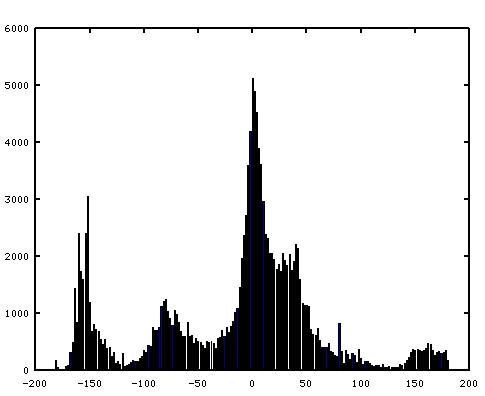
\includegraphics[scale=0.12]{figures/foreground_diff_h.png}}
        \hspace{0.05cm}
        \subfloat[]{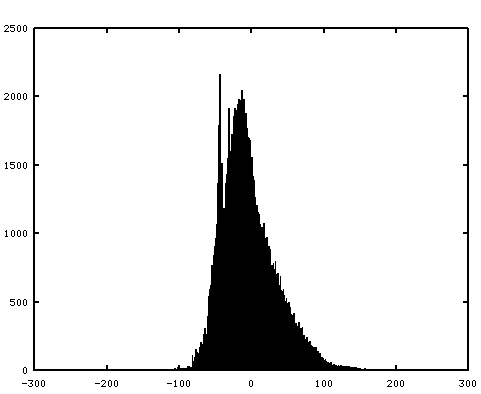
\includegraphics[scale=0.12]{figures/foreground_diff_s.png}}
        \hspace{0.05cm}
        \subfloat[]{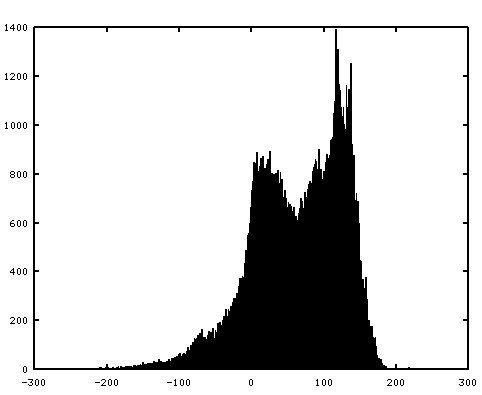
\includegraphics[scale=0.12]{figures/foreground_diff_v.png}}
        \caption{Example distributions over the difference in (a) hue, (b)
            saturation, and (c) value components for {\bf true object pixels},
            extracted from our hallway dataset.}
        \label{fig:foreground-distribution}
    \end{figure}

    \vspace{-0.3in}
    
    \begin{figure}
        \centering
        \subfloat[]{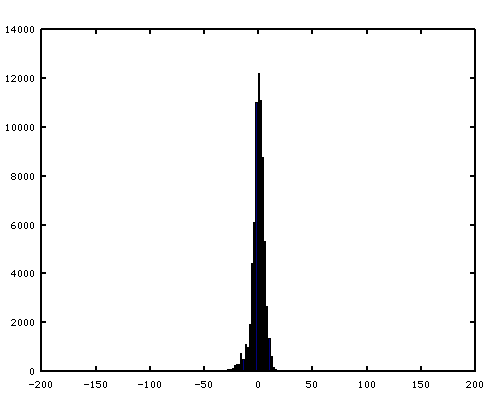
\includegraphics[scale=0.12]{figures/shadow_diff_h.png}}
        \hspace{0.05cm}
        \subfloat[]{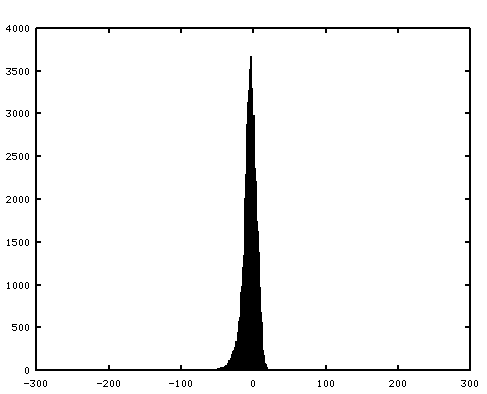
\includegraphics[scale=0.12]{figures/shadow_diff_s.png}}
        \hspace{0.05cm}
        \subfloat[]{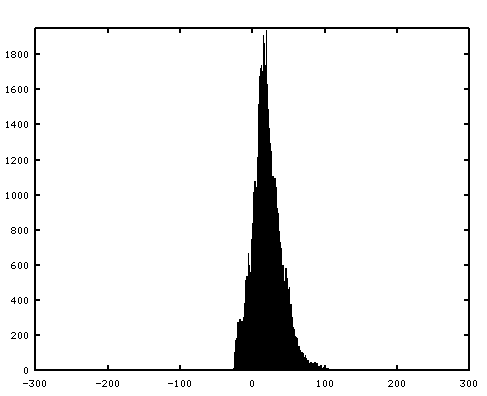
\includegraphics[scale=0.12]{figures/shadow_diff_v.png}}
        \caption{Example distributions over the difference in (a) hue, (b)
            saturation, and (c) value components for {\bf shadow pixels},
            extracted from our hallway dataset.}
        \label{fig:shadow-distribution}
    \end{figure}

\end{frame}

%--------------------------------------------------------------------

\begin{frame}
    \frametitle{ML Object/Shadow Discrimination}
    \framesubtitle{Measurement Likelihood for Shadow Pixels}

    We define the probability of measurement for pixel $(x, y)$ given its
    assignment as follows.
    \begin{equation*}
        \label{eq:shadow-measurement}
        \begin{array}{ccl}
            P(M_{\text{xy}} \mid A_{\text{xy}} = \text{sh}) 
                & = & P(H_{\text{diff}} \mid A_{\text{xy}} = \text{sh}) \times \\
                &   & P(S_{\text{diff}} \mid A_{\text{xy}} = \text{sh}) \times \\
                &   & P(V_{\text{diff}} \mid A_{\text{xy}} = \text{sh}),
        \end{array}
    \end{equation*}
    where $M_{xy}$ is a tuple containing the HSV value for pixel $(x,y)$
    in the current image as well as the HSV value for pixel $(x,y)$ in the
    background model for pixel $(x,y)$, and $A_{xy}$ is the assignment of
    pixel $(x,y)$ as object or shadow.  
    Similarly, the probability of measurement given its assignment 
    for object pixels can be computed as follows.
    \begin{equation*}
        \label{eq:foreground-measurement}
        \begin{array}{ccl}
            P(M_{\text{xy}} \mid A_{\text{xy}} = \text{obj}) 
                & = & P(H_{\text{diff}} \mid A_{\text{xy}} = \text{obj}) \times \\
                &   & P(S_{\text{diff}} \mid A_{\text{xy}} = \text{obj}) \times \\
                &   & P(V_{\text{diff}} \mid A_{\text{xy}} = \text{obj})
        \end{array}
    \end{equation*}
  
    Here ``sh'' stands for shadow and ``obj'' stands for object. 

\end{frame}

%--------------------------------------------------------------------

\ifnum\short=0

\begin{frame}
    \frametitle{ML Object/Shadow Discrimination}
    \framesubtitle{Measurement Likelihood for Shadow Pixels}

    To make the problem tractable, we assume that the distributions over 
    the components on the right hand side in the previous equation  
    follow Gaussian distributions, defined as follows.

    \begin{equation*}
        P(H_{\text{diff}} \mid A_{\text{xy}} = \text{sh}) =
        {\cal N}(H_{\text{diff}} ;
        \mu_{h_{\text{diff}}^{\text{sh}}},
        \sigma^2_{h_{\text{diff}}^{\text{sh}}})
    \end{equation*}
    \begin{equation*}
        P(S_{\text{diff}} \mid A_{\text{xy}} = \text{sh}) =
        {\cal N}(S_{\text{diff}} ;
        \mu_{s_{\text{diff}}^{\text{sh}}},
        \sigma^2_{s_{\text{diff}}^{\text{sh}}})
    \end{equation*}
    \begin{equation*}
        P(V_{\text{diff}} \mid A_{\text{xy}} = \text{sh}) =
        {\cal N}(V_{\text{diff}} ;
        \mu_{v_{\text{diff}}^{\text{sh}}},
        \sigma^2_{v_{\text{diff}}^{\text{sh}}})
    \end{equation*}

\end{frame}

%--------------------------------------------------------------------

\begin{frame}
    \frametitle{ML Object/Shadow Discrimination}
    \framesubtitle{Measurement Likelihood for Object Pixels}

    Similarly, the probability of measurement given its assignment 
    for object pixels can be computed as follows.
    \begin{equation*}
        \label{eq:foreground-measurement}
        \begin{array}{ccl}
            P(M_{\text{xy}} \mid A_{\text{xy}} = \text{obj}) 
                & = & P(H_{\text{diff}} \mid A_{\text{xy}} = \text{obj}) \times \\
                &   & P(S_{\text{diff}} \mid A_{\text{xy}} = \text{obj}) \times \\
                &   & P(V_{\text{diff}} \mid A_{\text{xy}} = \text{obj})
        \end{array}
    \end{equation*}
  
    Here ``obj'' stands for object. 

\end{frame}

%--------------------------------------------------------------------

\begin{frame}
    \frametitle{ML Object/Shadow Discrimination}
    \framesubtitle{Measurement Likelihood for Shadow Pixels}
  
    As for the shadow pixel distributions, we assume Gaussian distributions 
    over the components
    on the right hand side in the previous equation, as follows.

    \begin{equation*}
        P(H_{\text{diff}} \mid A_{\text{xy}} = \text{obj}) =
        {\cal N}(H_{\text{diff}} ;
        \mu_{h_{\text{diff}}^{\text{obj}}},
        \sigma^2_{h_{\text{diff}}^{\text{obj}}})
    \end{equation*}
    \begin{equation*}
        P(S_{\text{diff}} \mid A_{\text{xy}} = \text{obj}) =
        {\cal N}(S_{\text{diff}} ;
        \mu_{s_{\text{diff}}^{\text{obj}}},
        \sigma^2_{s_{\text{diff}}^{\text{obj}}})
    \end{equation*}
    \begin{equation*}
        P(V_{\text{diff}} \mid A_{\text{xy}} = \text{obj}) =
        {\cal N}(V_{\text{diff}} ;
        \mu_{v_{\text{diff}}^{\text{obj}}},
        \sigma^2_{v_{\text{diff}}^{\text{obj}}})
    \end{equation*}

\end{frame}

\fi

%--------------------------------------------------------------------

\begin{frame}
    \frametitle{ML Object/Shadow Discrimination}
    \framesubtitle{Model Parameters}

    We estimate the parameters \\

    \medskip
  
    $\Theta = \{
    \mu_{v_{\text{diff}}^{\text{sh}}},
    \sigma^2_{v_{\text{diff}}^{\text{sh}}},
    \mu_{v_{\text{diff}}^{\text{sh}}},
    \sigma^2_{v_{\text{diff}}^{\text{sh}}},
    \mu_{v_{\text{diff}}^{\text{sh}}},
    \sigma^2_{v_{\text{diff}}^{\text{sh}}},
    \mu_{v_{\text{diff}}^{\text{obj}}},
    \sigma^2_{v_{\text{diff}}^{\text{obj}}},
    \mu_{v_{\text{diff}}^{\text{obj}}},
    \sigma^2_{v_{\text{diff}}^{\text{obj}}},
    \mu_{v_{\text{diff}}^{\text{obj}}},
    \sigma^2_{v_{\text{diff}}^{\text{obj}}} \}$ \\

    \medskip
  
    directly from training data during the offline phase.

\end{frame}

%--------------------------------------------------------------------

\begin{frame}
    \frametitle{ML Object/Shadow Discrimination}
    \framesubtitle{Pixel Classification}
  
    In the \alert{online} phase:

    \medskip

    Given the model estimate $\Theta$, we use the
    maximum likelihood approach to classify a pixel as a shadow pixel if
    \begin{equation*}
        \label{eq:ml}
        P(M_{\text{xy}} \mid A_{xy}=\text{sh} ; \Theta ) >
        P(M_{\text{xy}} \mid A_{xy}=\text{obj} ; \Theta ).
    \end{equation*}
    Otherwise, we classify the pixel as an object pixel.
  
    \bigskip
  
    We could add the prior probabilities to the shadow model
    and the object model in the equation above to obtain a maximum a 
    posteriori classifier. In our experiments, we assume equal priors.

\end{frame}

%--------------------------------------------------------------------

\begin{frame}
    \frametitle{ML Object/Shadow Discrimination}
    \framesubtitle{Experimental Results}

    We present experimental results for
    \begin{enumerate}
        \item our proposed maximum likelihood (ML) classification method; 
        \item the deterministic nonmodel-based (DNM) method;
        \item the normalized cross-correlation (NCC) method.
    \end{enumerate}

\end{frame}

%--------------------------------------------------------------------

\begin{frame}
    \frametitle{ML Object/Shadow Discrimination}
    \framesubtitle{Experimental Results (cont.)}

    We performed the experiments on three video sequences. The figure 
    below shows sample frames from the three video sequences.
  
    \begin{figure}
        \centering
        \subfloat[]{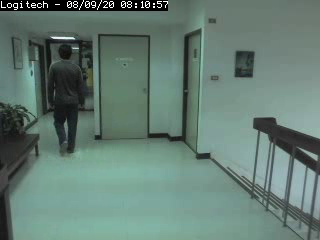
\includegraphics[scale=0.25]{figures/csim_hallway_benchmark.png}}
        \hspace{0.05cm}
        \subfloat[]{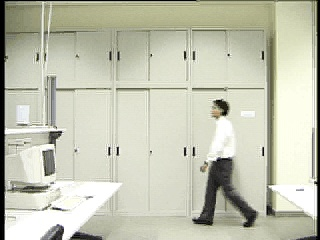
\includegraphics[scale=0.25]{figures/aton_lab_benchmark.png}}
        \hspace{0.05cm}
        \subfloat[]{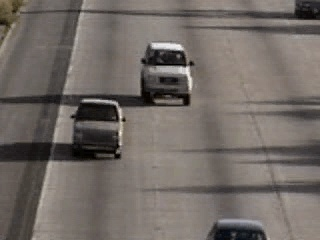
\includegraphics[scale=0.25]{figures/aton_highway1_benchmark.png}}
        \caption{Sample frames from the (a) Hallway, (b) Laboratory, and (c)
            Highway video sequences}
        \label{fig:benchmark}
    \end{figure}

    The {\em Hallway} sequence is our own dataset. The {\em Laboratory} and 
    {\em Highway} sequences were first introduced in Prati et al.\ (2003).

\end{frame}

%--------------------------------------------------------------------

\begin{frame}
    \frametitle{ML Object/Shadow Discrimination}
    \framesubtitle{Experimental Results (cont.)}

    To evaluate the performance of the methods, we compute the two 
    metrics proposed by Prati et al.\ (2003), defining the shadow 
    detection rate $\eta$ and the shadow discrimination rate $\xi$ 
    as follows:

    \[
        \eta = \frac{TP_{\text{sh}}}{TP_{\text{sh}} + FN_{\text{sh}}};\; 
        \xi = \frac{TP_{\text{obj}}}{TP_{\text{obj}} + FN_{\text{obj}}},
    \]
    where the subscript ``sh'' and ``obj'' stand for shadow and object,
    respectively. $TP$ and $FN$ are the number of true positive (i.e., the
    shadow or object pixels correctly identified) and false negative
    (i.e., the shadow or object pixels classified incorrectly) pixels.

\end{frame}

%--------------------------------------------------------------------

\ifnum\short=0

\begin{frame}
    \frametitle{ML Object/Shadow Discrimination}
    \framesubtitle{Experimental Results (cont.)}

    More information about $\eta$ and $\xi$ 
    \begin{itemize}
        \item $\eta$: the proportion of shadow pixels 
            correctly detected
        \item $\xi$: the proportion of object pixels 
            correctly detected.  
    \end{itemize}  
    
    $\eta$ and $\xi$ can also be thought of as the true
    positive rate (sensitivity) and true negative rate (specificity) for
    detecting shadows, respectively. 
  
    \bigskip
  
    In the experiment, we also compare the methods with the additional 
    two metrics: precision and $F_1$ score.

\end{frame}

\fi

%--------------------------------------------------------------------

\begin{frame}
    \frametitle{ML Object/Shadow Discrimination}
    \framesubtitle{Experimental Results (cont.)}

    Ground truth data:
    \begin{itemize}
        \item The {\em Laboratory} and {\em Highway} video sequences are 
            provided in Sanin et al.\ (2012).
        \item A standard Gaussian mixture (GMM) background model in used to 
            extract 
            foreground pixels. 
        \item For our {\em Hallway} video sequence, we used the previously 
            mentioned extended version of the GMM background model for 
            foreground extraction, but the results were not substantially 
            different from those of the standard GMM.
    \end{itemize}

\end{frame}

%--------------------------------------------------------------------

\ifnum\short=0

\begin{frame}
    \frametitle{ML Object/Shadow Discrimination}
    \framesubtitle{Experimental Results (cont.)}

    We performed five-fold cross validation to find the best parameters 
    for each model for each of the three models and each of the three 
    data sets.

    \bigskip

    Varied the parameter settings for each method on each video dataset 
    and selected the setting that maximized the $F_1$ score (a measure 
    combining both precision and recall) over the cross validation test 
    sets.

\end{frame}

\fi

%--------------------------------------------------------------------

\begin{frame}
    \frametitle{ML Object/Shadow Discrimination}
    \framesubtitle{Experimental Results (cont.)}

    \begin{table}
        \caption{Comparison of shadow detection results between the
            proposed, DNM, and NCC methods.}
        \label{tab:comparison-results}
        \vspace{-0.2in}
        \centering
        \begin{figure}
            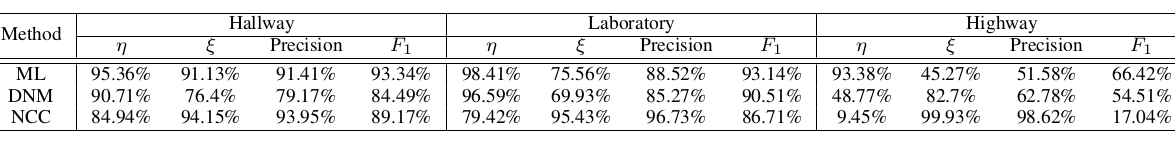
\includegraphics[width=4.85in]{figures/shadow-detection-results.png}
        \end{figure}
    \end{table}
    
    From the table, our proposed method
    \begin{itemize}
        \item achieves the top performance for shadow detection 
            rate $\eta$ and $F_1$ score in every case; 
        \item obtains good shadow discrimination rate $\xi$ in every case.
    \end{itemize}

\end{frame}

%--------------------------------------------------------------------

\begin{frame}
    \frametitle{ML Object/Shadow Discrimination}
    \framesubtitle{Experimental Results (cont.)}

    The DNM method has stable performance for all three videos, with good 
    performance for all metrics.

    \bigskip

    Both the DNM method and our proposed method suffer from the problem that 
    the object colors can be confused with the background color. We clearly 
    see this situation in the {\em Highway} sequence (third row in the 
    next figure).

    \bigskip
  
    The NCC method achieves the best shadow discrimination rate $\xi$ and 
    precision  because it classifies nearly every pixel as object as can be 
    seen in the next figure.

\end{frame}

%--------------------------------------------------------------------

\begin{frame}
    \frametitle{ML Object/Shadow Discrimination} 
    \framesubtitle{Experimental Results (cont.)} 

    \begin{figure}
        \centering
        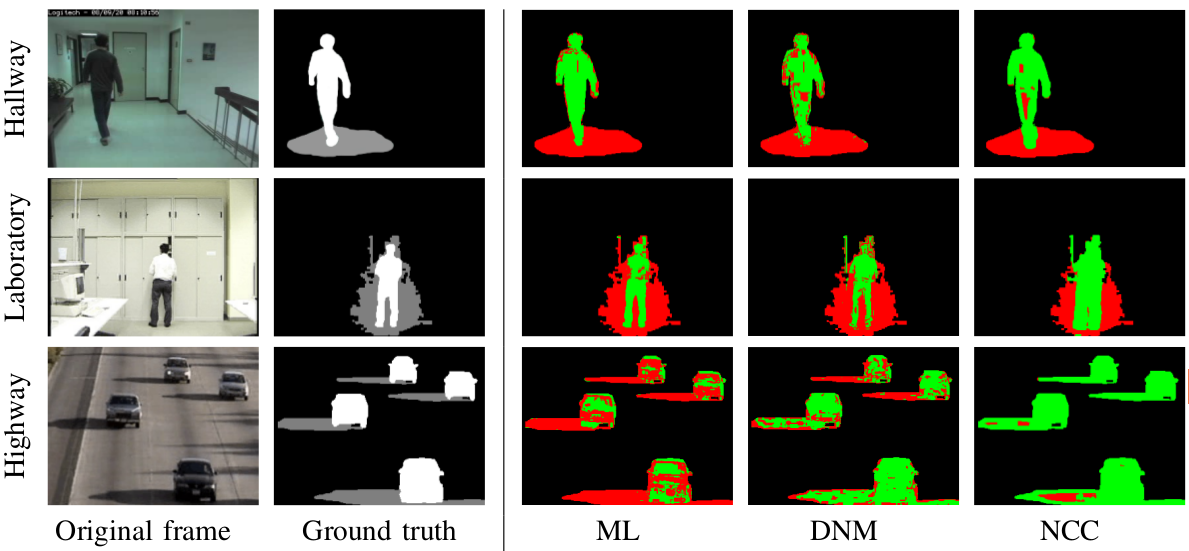
\includegraphics[width=4in]{figures/shadow-detection-results-for-an-arbitrary-frame.png}
        \vspace{-0.1in}
        \caption{Results for an arbitrary frame in each video sequence. The
            first column contains an example original frame for each video
            sequence. The second column shows the ground truth for that frame,
            where object pixels are labeled in white and shadow pixels are
            labeled in gray. The remaining columns show shadow detection
            results for each method, where pixels labeled as object shown in
            green and pixels labeled as shadow are shown in red.}
        \label{fig:results-for-arbitrary-frame}
    \end{figure}

\end{frame}

%--------------------------------------------------------------------

\begin{frame}
    \frametitle{ML Object/Shadow Discrimination}
    \framesubtitle{Conclusion}

    \begin{itemize}
        \item We propose a new method for detecting shadows using a simple 
            maximum likelihood approach based on color information;
        \item We extend the deterministic nonmodel-based approach, designing 
            a parametric statistical model-based approach;
        \item Our experimental results show that our proposed method is 
            extremely effective and superior to the standard methods on three 
            different real-world video surveillance data sets.
    \end{itemize}

\end{frame}

%--------------------------------------------------------------------

\begin{frame}
    \frametitle{ML Object/Shadow Discrimination}
    \framesubtitle{Discussion}

    \begin{itemize}
        \item In some cases, our method misdetects shadow pixels due to 
            similar color between the object and the background and unclear 
            background texture in shadow regions;
        \item Incorporating geometric or shadow region shape priors would 
            potentially improve the detection and discrimination rates;
        \item We plan to address these issues, further explore the feasibility 
            of combining our method with other useful shadow features, and 
            integrate our shadow detection module with a real-world open source 
            video surveillance system.
    \end{itemize}

\end{frame}

